\section{Generality and Robustness}
\label{sec:generality}

Our main study fixes one small model and one dataset. We now probe whether the
two load-bearing findings---(i) deduplication does not help, and (ii) reasoning,
especially temporal, is a floor retrieval cannot cross---survive a change of
judge, a change of dataset, and a change of answerer.

\paragraph{A second, independent judge.} We re-judge the cached answers with a
different model, \texttt{llama3.2:3b} (vs.\ \texttt{qwen3:8b}). The two judges
agree on $81.3\%$ of $600$ items (Cohen's $\kappa = 0.52$, moderate);
\texttt{llama3.2} is stricter (positive rate $0.19$ vs.\ $0.31$). Crucially, the
\emph{policy ordering is identical} under the second judge: naive-dedup remains
dominated at every budget ($0.06$--$0.09$ vs.\ full $0.23$--$0.30$) and
query-aware $\approx$ full. Finding (i) is judge-robust; only the absolute scale
shifts.

\paragraph{A second dataset (LongMemEval).} We test finding (ii) on the
LongMemEval~\cite{wu2024longmemeval} oracle split, which supplies gold evidence
sessions per question, typed by reasoning kind. Answering from gold evidence
with \texttt{qwen3:8b} (Table~\ref{tab:lme}, Fig.~\ref{fig:lme}),
\emph{temporal-reasoning is the lowest type} ($0.275$), far below easy
single-session types ($0.80$--$0.95$), with multi-session (the multi-hop analog)
second-lowest ($0.375$). This mirrors LoCoMo, where temporal is also the worst
category with gold evidence ($0.156$). The temporal floor is not a LoCoMo
artifact: it replicates across two datasets and two question taxonomies.

\begin{table}[t]
\centering
\small
\begin{tabular}{lcc}
\toprule
question type & oracle acc. & $n$ \\
\midrule
single-session-assistant & 0.950 & 40 \\
single-session-user & 0.800 & 40 \\
knowledge-update & 0.600 & 40 \\
single-session-preference & 0.467 & 30 \\
multi-session & 0.375 & 40 \\
\textbf{temporal-reasoning} & \textbf{0.275} & 40 \\
\midrule
overall & 0.583 & 230 \\
\bottomrule
\end{tabular}
\caption{LongMemEval (oracle split), \texttt{qwen3:8b} answering from gold
evidence. Temporal reasoning is the floor even with perfect evidence,
replicating the LoCoMo result on a second dataset.}
\label{tab:lme}
\end{table}

\begin{figure}[t]
\centering
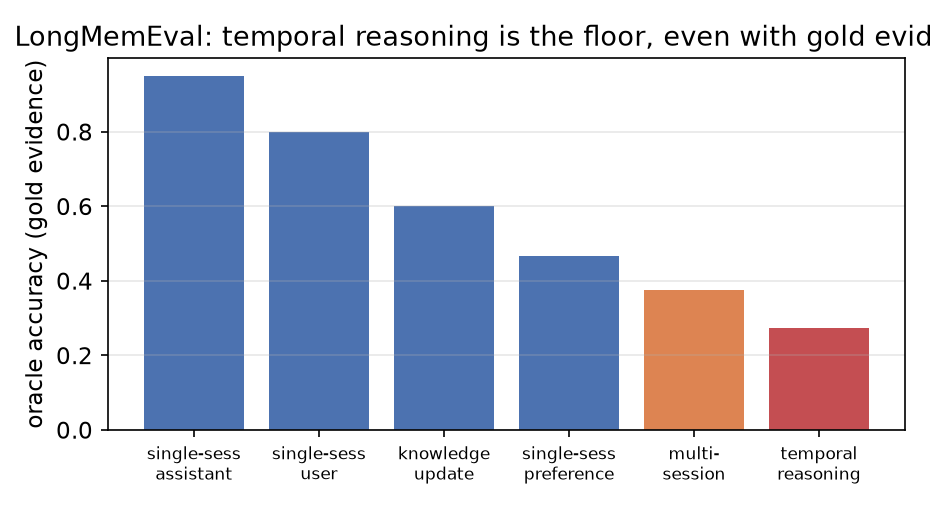
\includegraphics[width=\linewidth]{figures/fig_longmemeval.png}
\caption{LongMemEval oracle-answering accuracy by question type. Temporal
reasoning (right, red) is lowest despite gold evidence.}
\label{fig:lme}
\end{figure}

\paragraph{A second answerer model.} Finally we replace the answering model with
\texttt{llama3.2:3b} (retrieval and the qwen3-built store held fixed; judge held
fixed as \texttt{qwen3:8b}), at $k{=}8$ on $n{=}120$ questions per policy. The
ordering again replicates: naive-dedup is dominated ($0.192$ vs.\ full $0.342$)
and query-aware $\approx$ full ($0.333$). Finding (i) survives a change of the
generation model as well as the judge.

\paragraph{Summary.} The two load-bearing findings are robust to the axes we
could vary locally: deduplication fails to help under two judges and two
answerer models, and the temporal-reasoning floor appears under two datasets.
Absolute accuracies shift with model and judge; the qualitative conclusions do
not.
